
\documentclass[11pt]{article}
\usepackage[margin=0.8in]{geometry}
\usepackage{amsmath,amssymb,booktabs,array,longtable}
\usepackage{hyperref}
\usepackage{enumitem}
\usepackage{graphicx}
\usepackage{float}
\setlist{nosep}

\begin{document}

\begin{center}
{\Large\textbf{Shiv Nadar University Chennai}}\\
\textbf{CS3807 -- Deep Learning Laboratory}\\
\textbf{Experiment 2}\\
{\large\textbf{Implementation of a Multi-Layer Perceptron (MLP) for Multi-Class Image Classification}}
\end{center}

\renewcommand{\arraystretch}{1.25}

\begin{flushleft}
\textbf{Name:} Johan Emmanuel S\\
\textbf{Registration Number:} 24011101043\\
\end{flushleft}

\begin{tabular}{|p{3.8cm}|p{8cm}|p{2cm}|}
\hline
Degree \& Branch & B.Tech Artificial Intelligence \& Data Science & Semester V\\ \hline
Subject Code \& Name & CS3807 -- Deep Learning Laboratory & AY: 2026--27\\ \hline
\end{tabular}

\section*{1. Objective}
Implement an MLP using TensorFlow/Keras on the Fashion-MNIST dataset. Learn image preprocessing, flattening, model construction, training, evaluation, and automated hyperparameter optimization.

\section*{2. Background Theory}
An MLP consists of an input layer, hidden layers and an output layer.

\[
z^{(l)}=W^{(l)}a^{(l-1)}+b^{(l)},\qquad
a^{(l)}=f(z^{(l)})
\]

Output layer:
\[
\hat y=\mathrm{Softmax}(z)
\]

Loss:
\[
L=-\sum_i y_i\log(\hat y_i)
\]

Recommended architecture:

\begin{center}
784 $\rightarrow$ Dense(128, ReLU) $\rightarrow$ Dense(64, ReLU) $\rightarrow$ Dense(10, Softmax)
\end{center}

\section*{3. Dataset}
Dataset: Fashion-MNIST

Training Images: 60,000 \\
Testing Images: 10,000 \\
Classes: 10 \\
Image Size: $28\times28$

\section*{4. Image Preprocessing}

Fashion-MNIST images are stored as $28\times28$ matrices. Dense layers require a one-dimensional feature vector.

\[
28\times28=784
\]

Example:

\[
\begin{bmatrix}
10&20\\30&40
\end{bmatrix}
\rightarrow
[10,20,30,40]
\]

Perform the following preprocessing:

\begin{enumerate}
\item Load Fashion-MNIST.
\item Display sample images.
\item Flatten images.
\item Normalize pixels to [0,1].
\item Convert labels into one-hot vectors.
\end{enumerate}

\section*{5. Experimental Procedure}

\textbf{Task 1: Dataset Exploration}
\begin{itemize}
\item Load Fashion-MNIST.
\item Print dataset dimensions.
\item Display ten sample images.
\item Plot class distribution.
\end{itemize}

\textbf{Expected Output:}
Dataset summary and sample images.

\bigskip

\textbf{Task 2: Data Preprocessing}

\begin{itemize}
\item Flatten images.
\item Normalize pixel values.
\item Print tensor shapes before and after preprocessing.
\end{itemize}

\bigskip

\textbf{Task 3: Model Construction}

Construct an MLP with

\begin{itemize}
\item Input layer (784)
\item Dense(128, ReLU)
\item Dense(64, ReLU)
\item Dense(10, Softmax)
\end{itemize}

Display \texttt{model.summary()}.

\bigskip

\textbf{Task 4: Model Training}

Compile using

\begin{itemize}
\item Optimizer: Adam
\item Loss: Categorical Cross Entropy
\item Metric: Accuracy
\end{itemize}

Train for 20 epochs with batch size 32.

\bigskip

\textbf{Task 5: Model Evaluation}

Compute

\begin{itemize}
\item Accuracy
\item Precision
\item Recall
\item F1-score
\item Confusion Matrix
\item Classification Report
\end{itemize}

\section*{6. Source Code}
The source code for the Multi Layer Perceptron with analysis and Hyperparameter Tuning can be found at \url{https://github.com/faultybyte/deep-learning-lab}

\section*{7. Hyperparameter Optimization}

Instead of manually selecting hyperparameters, students shall perform automated hyperparameter optimization using either \textbf{GridSearchCV} or \textbf{RandomizedSearchCV} (recommended) together with the SciKeras wrapper.

Optimize the following search space.

\begin{center}
\begin{tabular}{|p{5cm}|p{7cm}|}
\hline
Hyperparameter & Candidate Values\\
\hline
Hidden Layers & 1, 2, 3\\
Hidden Neurons & 32, 64, 128, 256\\
Learning Rate & 0.1, 0.01, 0.001\\
Batch Size & 16, 32, 64, 128\\
Epochs & 10, 20, 30\\
Optimizer & SGD, Adam, RMSProp\\
Activation Function & ReLU, Tanh, Sigmoid\\
Dropout Rate (Optional) & 0.0, 0.2, 0.5\\
\hline
\end{tabular}
\end{center}

\subsection*{Tasks}

\begin{enumerate}
\item Build a baseline MLP model.
\item Define the hyperparameter search space.
\item Perform Grid Search or Randomized Search using 5-fold cross-validation.
\item Record the best hyperparameter combination.
\item Retrain the model using the optimized hyperparameters.
\item Evaluate the optimized model on the testing dataset.
\item Compare the optimized model with the baseline model.
\end{enumerate}

\section*{8. Results}

\textbf{Best Hyperparameters}

\begin{tabular}{|p{6cm}|p{6cm}|}
\hline
Hidden Layers & 1\\\hline
Hidden Neurons & 256\\\hline
Learning Rate & 0.001\\\hline
Batch Size & 64\\\hline
Optimizer & adam\\\hline
Activation Function & tanh\\\hline
Epochs & 20\\\hline
Dropout & 0.2\\\hline
Cross-validation Accuracy & 0.8896\\\hline
Testing Accuracy & 0.8726\\\hline
\end{tabular}

\vspace{3mm}

\textbf{Performance Comparison}

\begin{tabular}{|p{4cm}|c|c|}
\hline
Metric & Baseline & Optimized\\
\hline
Accuracy & 0.8497 & 0.8726\\
Precision & 0.8578 & 0.8709\\
Recall & 0.8497 & 0.8692\\
F1-score & 0.8479 & 0.8685\\
Training Time & 1.3 min & 1.9 min \\
\hline
\end{tabular}

\section*{9. Plots with Inference}

\subsection{Sample Images}
\begin{figure}[H]
\centering
\includegraphics[width=0.75\textwidth]{mnist_sample_images.eps}
\caption{Representative sample images from the Fashion-MNIST dataset with class labels.}
\label{fig:sample_images}
\end{figure}

\textbf{Inference:} Visualizing the first ten raw samples reveals the $28 \times 28$ pixel grayscale resolution and structural characteristics of the garment images. Complex shapes like Pullovers and Shirts exhibit higher feature overlap, indicating potential classification confusion.

\subsection{Class Distribution}
\begin{figure}[H]
\centering
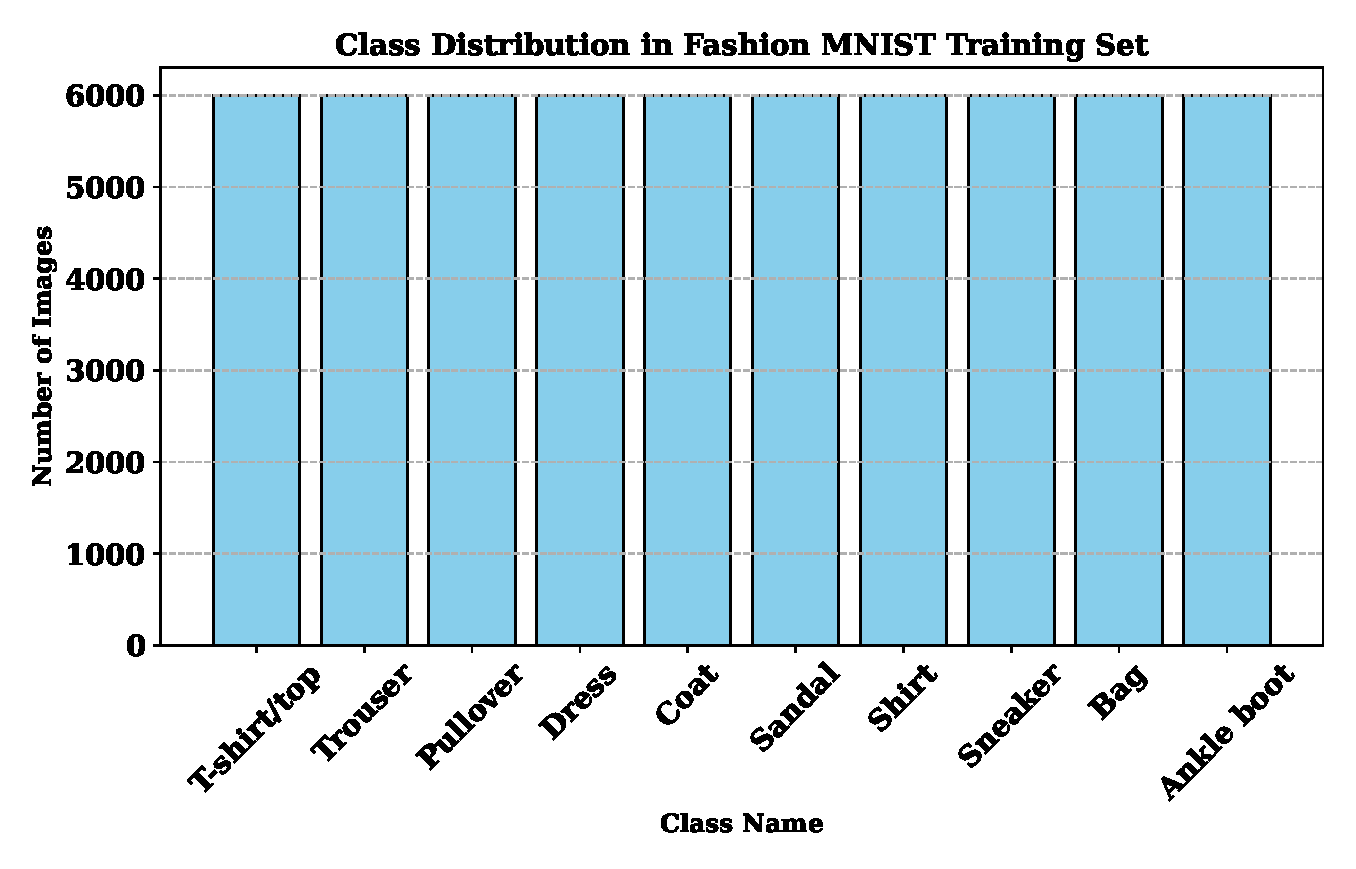
\includegraphics[width=0.65\textwidth]{mnist_class_distribution.eps}
\caption{Class frequency distribution across the Fashion-MNIST training dataset.}
\label{fig:class_dist}
\end{figure}

\textbf{Inference:} The bar chart confirms that the Fashion-MNIST dataset is perfectly balanced, containing exactly 6,000 training samples per class across all 10 categories. Therefore, baseline accuracy serves as an unbiased metric.

\subsection{Training vs. Validation Accuracy}
\begin{figure}[H]
\centering
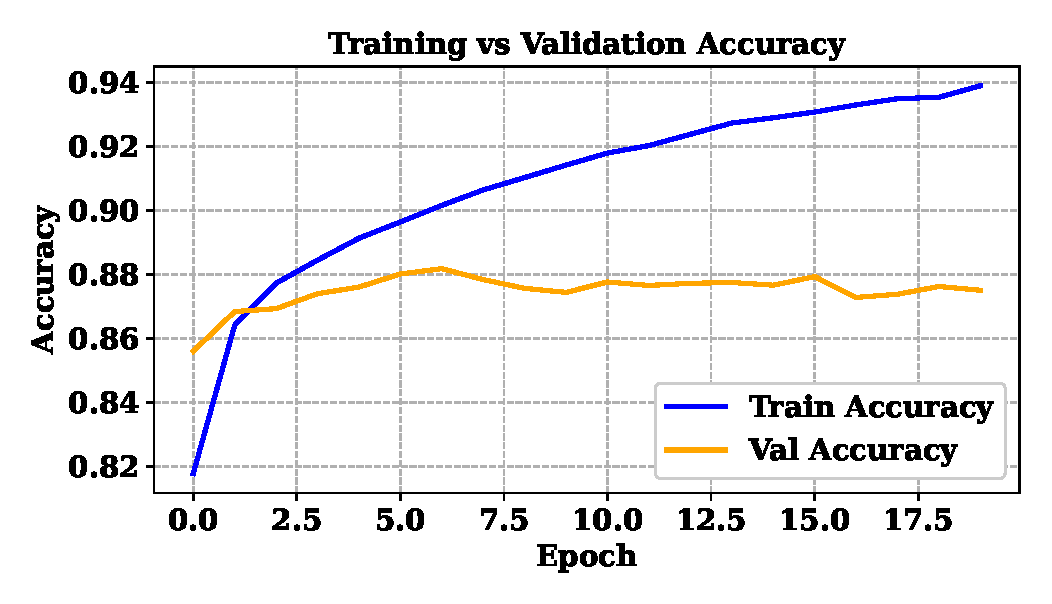
\includegraphics[width=0.65\textwidth]{accuracy_curve.eps}
\caption{Training vs. Validation Accuracy trajectory across training epochs.}
\label{fig:acc_curve}
\end{figure}

\textbf{Inference:} Training accuracy continually increases towards 0.94, whereas validation accuracy plateaus near 0.88 after epoch 5. This plateau indicates that the network reaches its optimal generalization capacity early, beyond which further training yields diminishing returns.

\subsection{Training vs. Validation Loss}
\begin{figure}[H]
\centering
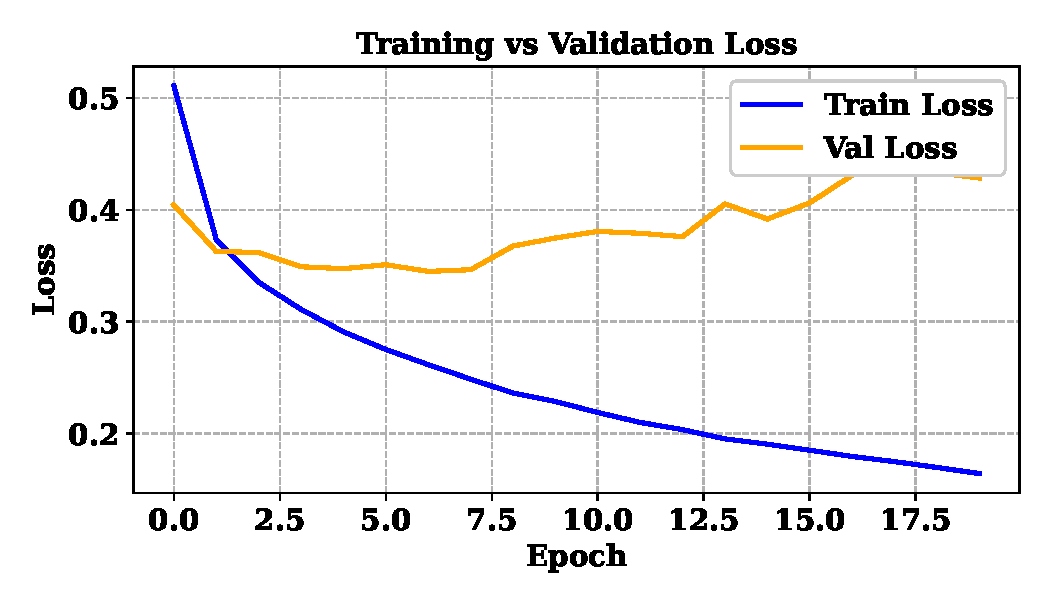
\includegraphics[width=0.65\textwidth]{loss_curve.eps}
\caption{Training vs. Validation Categorical Cross-Entropy Loss over training epochs.}
\label{fig:loss_curve}
\end{figure}

\textbf{Inference:} Training loss decreases smoothly toward 0.16, while validation loss bottoms out at epoch 5 and gradually rises to 0.43. This widening gap confirms the onset of overfitting in later epochs.

\subsection{Confusion Matrix}
\begin{figure}[H]
\centering

\includegraphics[width=0.7\textwidth]{confusion_matrix.eps}
\caption{Confusion Matrix Heatmap evaluated on the test set.}
\label{fig:confusion_matrix}
\end{figure}

\textbf{Inference:} The model shows high accuracy on distinct classes like Trousers (980) and Bags (970), but frequently confuses visually similar upper-body garments like Shirts, T-shirts, and Pullovers. This reflects the limitation of 1D flattened dense layers in capturing complex, overlapping spatial textures.

\subsection{Hyperparameter Search Results}
\begin{figure}[H]
\centering
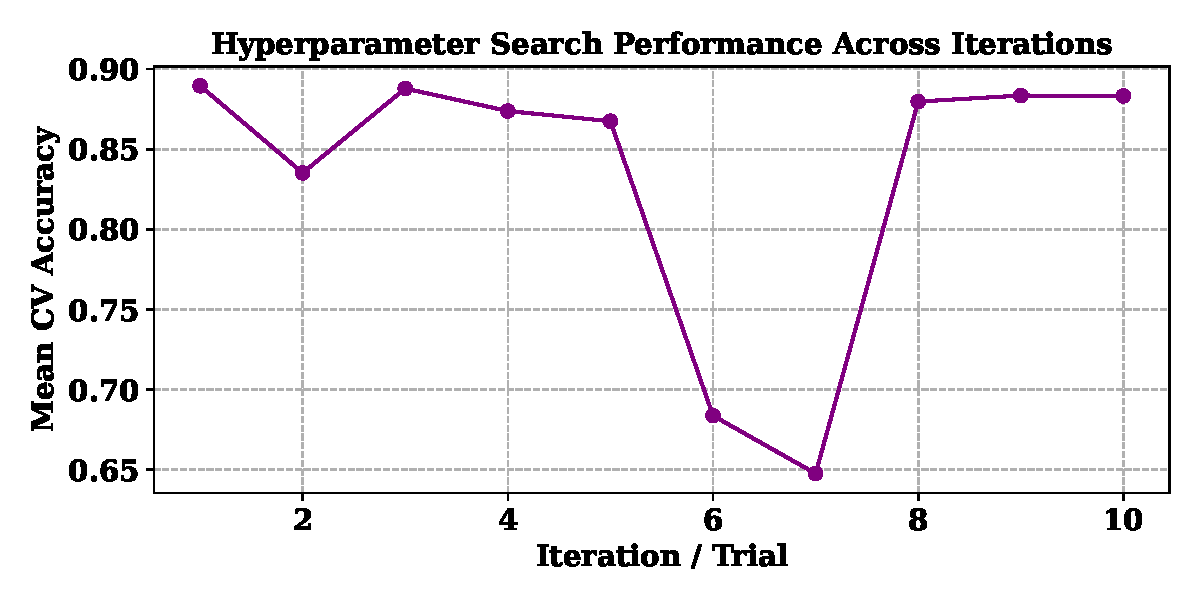
\includegraphics[width=0.65\textwidth]{hyperparameter_results.eps}
\caption{Mean Cross-Validation Accuracy score across evaluated candidate iterations.}
\label{fig:hp_results}
\end{figure}

\textbf{Inference:} CV accuracy varies significantly between 0.65 and 0.89 across trials, demonstrating high model sensitivity to hyperparameter choices. Sub-optimal configurations (trials 6 and 7) dropped performance sharply, while optimal parameters consistently achieved peak accuracies near 0.89.

\subsection{Best Model Accuracy Comparison}
\begin{figure}[H]
\centering
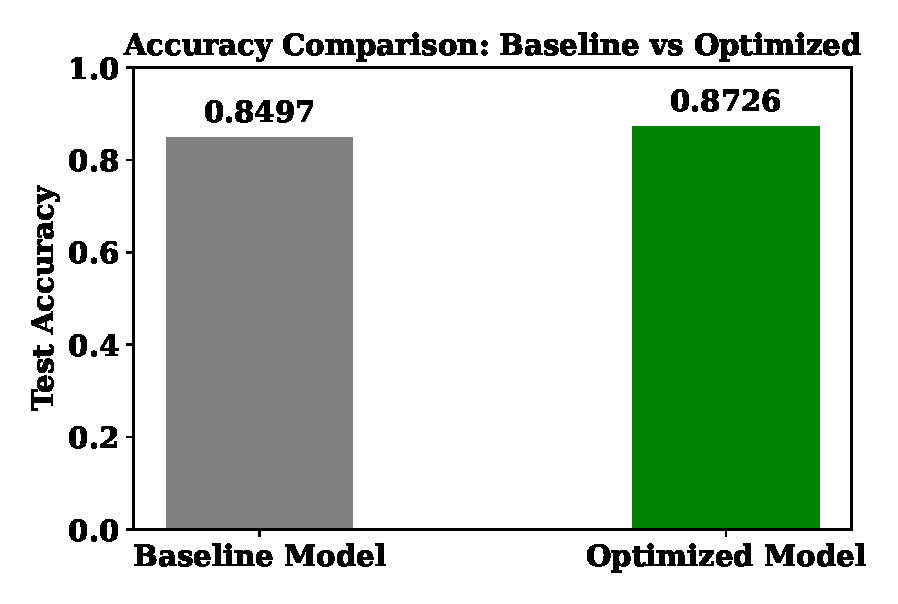
\includegraphics[width=0.5\textwidth]{accuracy_comparison.eps}
\caption{Comparative performance chart: Baseline MLP vs. Optimized MLP Model.}
\label{fig:model_comp}
\end{figure}

\textbf{Inference:} Automated hyperparameter optimization improved test accuracy from 0.8497 (baseline) to 0.8726. This 2.29\% performance lift proves that systematically tuning parameters like layer width, learning rate, and batch size enhances model generalization.

\section*{10. Discussion}

\begin{enumerate}
    \item \textbf{Which optimization method was used?} \\
    Automated optimization was performed using Scikit-Learn's \texttt{RandomizedSearchCV} with 5-fold cross-validation. It sampled 10 random hyperparameter combinations to evaluate models efficiently without the heavy compute cost of a full grid search.

    \item \textbf{Which hyperparameters were selected?} \\
    The best model used 1 hidden layer with 256 neurons, Tanh activation, and 0.2 dropout. It was trained using the Adam optimizer ($\text{learning rate} = 0.001$), a batch size of 64, and 20 epochs.

    \item \textbf{Did optimization improve performance?} \\
    Yes. Test accuracy increased from 84.97\% (baseline) to 87.26\%, proving that tuning layer width, activation functions, and regularization improves overall model generalization.

    \item \textbf{Which hyperparameter had the greatest impact?} \\
    The optimizer and learning rate had the largest impact. High learning rates (e.g., 0.1) or basic SGD struggled to converge, whereas Adam at 0.001 consistently delivered peak cross-validation accuracy.

    \item \textbf{Compare Grid Search and Randomized Search.} \\
    Grid Search checks every possible combination, guaranteeing the exact best setup in the grid but taking significantly longer. Randomized Search tests a random sample of combinations, finding a nearly identical top-performing setup in a fraction of the time.

    \item \textbf{Recommend the best MLP configuration.} \\
    The recommended setup for Fashion-MNIST is a single hidden layer with 256 units, Tanh activation, and 0.2 Dropout, trained using the Adam optimizer ($\text{lr} = 0.001$) with a batch size of 64 for 20 epochs.
\end{enumerate}

\section*{11. Conclusion}
In this experiment, a baseline Multi Layer Perceptron was built and trained on the Fashion MNIST dataset. Hyperparameter optimization was performed to select the best hyperparameters for the model.

\section*{12. References}
\begin{enumerate}
\item Goodfellow et al., \emph{Deep Learning}.
\item Bishop, \emph{Pattern Recognition and Machine Learning}.
\item Haykin, \emph{Neural Networks and Learning Machines}.
\item Fashion-MNIST Dataset.
\item TensorFlow/Keras Documentation.
\end{enumerate}

\end{document}
